% Declare evaluation floats early so IEEE two-column placement can keep them near their sections.

\begin{figure*}[t]
\centering
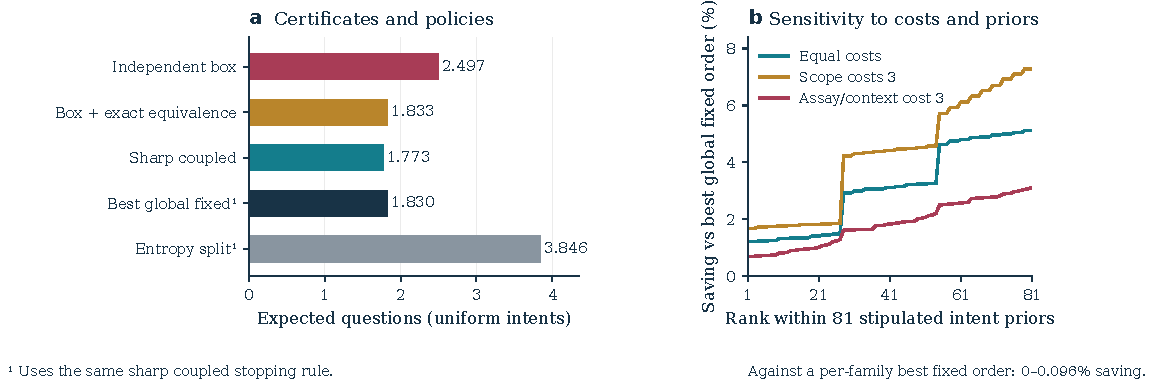
\includegraphics[width=\textwidth]{04_planning.pdf}
\caption{(a) Expected question counts under different certificates and policies. The fixed-order and entropy policies use the same sharp coupled graph; the box comparators optimize their own conservative stopping graphs. (b) The 81 priors in each cost scenario are ranked separately by saving against the hindsight-best global fixed order. These are stipulated sensitivity scenarios, not observed dialogue outcomes. The much stronger per-family fixed comparator nearly eliminates the adaptive advantage.}
\label{fig:planning}
\end{figure*}

\begin{figure*}[t]
\centering
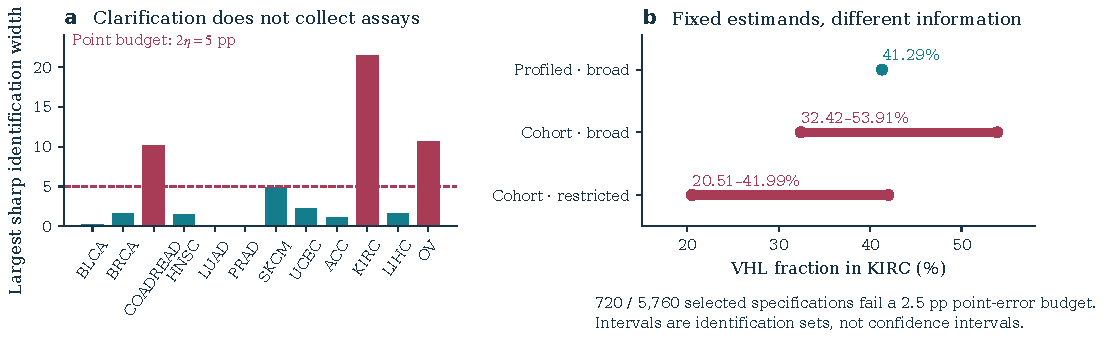
\includegraphics[width=\textwidth]{06_identification.pdf}
\caption{The point guard remains necessary after all intent fields are resolved. (a) Largest sharp interval width by TCGA cohort; the dashed threshold is twice the 2.5 pp minimax point-error budget. (b) KIRC--VHL examples distinguish a fixed profiled fraction from wide cohort-completion intervals. Exactly 720 selected TCGA specifications fail the point budget; this is a registry count, not an observed user failure rate.}
\label{fig:identification}
\end{figure*}

\begin{figure*}[t]
\centering
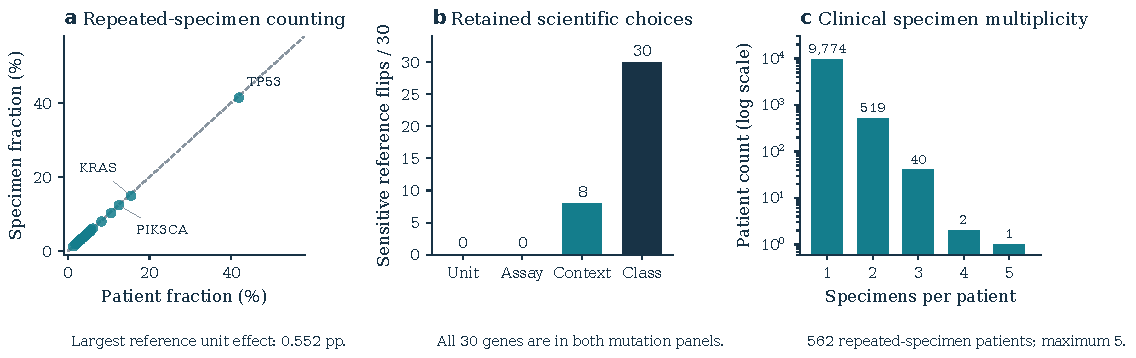
\includegraphics[width=\textwidth]{08_targeted_assay.pdf}
\caption{Separate MSK-IMPACT 2017 stress test, retaining all 30 panel genes. (a) Recorded patient and specimen fractions remain near the diagonal despite repeated specimens. (b) Sensitive reference-axis flips under the primary tolerance. All selected genes are in both source panels, so observed and completion-aware certificates coincide. (c) Patient specimen multiplicity on a logarithmic count axis; 562 patients have two or more specimens. These results challenge counting semantics while exposing the absence of empirical gene-panel missingness in this selected panel.}
\label{fig:msk}
\end{figure*}

\begin{figure*}[t]
\centering
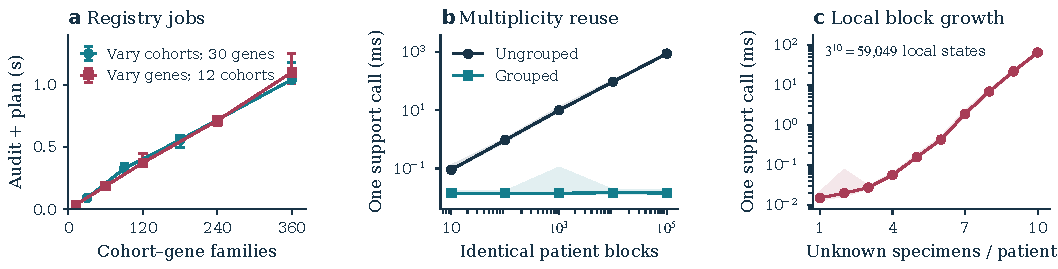
\includegraphics[width=\textwidth]{09_scaling.pdf}
\caption{Measured serial scaling; medians and min--max ranges over five warmed repetitions. (a) Exact certificate-and-planner jobs on prefixes of the frozen cohort/gene lists, after table preparation. (b) Synthetic identical patient tables isolate multiplicity grouping for one integer support. (c) One synthetic repeated-unprofiled patient isolates the retained local exponential cost. Panels time different operations and are not directly comparable. No synthetic rows are new biological evidence.}
\label{fig:scaling}
\end{figure*}
